\chapter{Теоретическое введение}
	\label{chap:one}
\section{Сети Петри}

Формально сеть Петри определена в~\cite{piterson} и представляет собой двудольный граф с двумя родами вершин: одни вершины называются позициями, другие
называются переходами. 
Построение моделей систем в виде сетей Петри заключается в следующем.
\begin{enumerate}
	\item 	Моделируемые процессы описываются множеством событий (действий) и условий определяющих возможность наступления этих событий, а также причинно-следственными отношениями, устанавливаемыми на множестве пар "события-условия".
	\item Определяются события-действия, последовательность выполнения которых управляется состояниями системы. Состояния системы задаются множеством условий, формируемых в виде предикатов. Количественно условия характеризуются величиной, которая выражается числами натурального ряда.
\item Условия, в зависимости от значений их количественных характеристик, могут выполняться или нет. Выполнение условий обеспечивает возможность реализации событий. Условия, с фактом выполнения которых связывается возможность реализации событий, называются предусловиями. Реализация события обеспечивает возможность выполнения других условий, находящихся с предусловиями в причинно-следственной связи. Эти условия называются постусловиями.
\end{enumerate}

В сетях Петри условия - это позиции, а события - переходы. В соответствии с этим граф сети Петри является двудольным ориентированным мультиграфом. Изображение позиции и перехода на графе показано на рисунке \ref{img:example}.

\begin{figure}[h!]
	\begin{minipage}[ht]{0.49\linewidth}
		\center{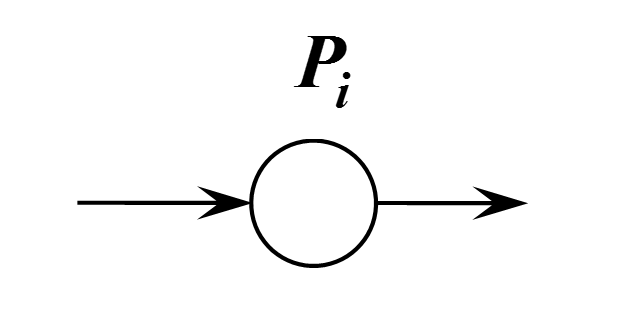
\includegraphics[width=0.3\textwidth]{place} \\ а)}
	\end{minipage}
	\hfill
	\begin{minipage}[ht]{0.49\linewidth}
		\center{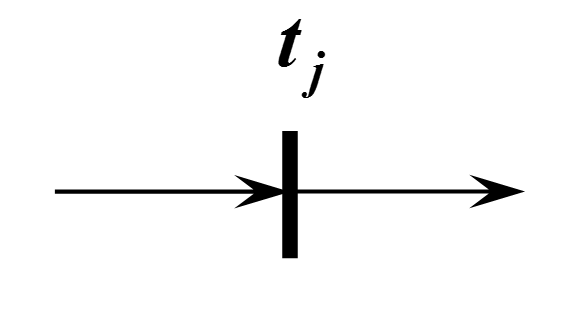
\includegraphics[width=0.3\linewidth]{tansition} \\ б)}
	\end{minipage}
	\caption{a) "--- Изображение позиции, б) "--- Изображение перехода. }
	\label{img:example}  
\end{figure}

Ориентированные дуги могут соединять только позиции и переходы в прямом и обратном направлении (свойство двудольности~\cite{piterson}). Сеть Петри является мультиграфом, так как допускается кратность дуг между позициями и переходами (вершинами графа). Пример сети Петри приведен на рисунке \ref{img:petri-net}.

\begin{figure}[h!]
	\center{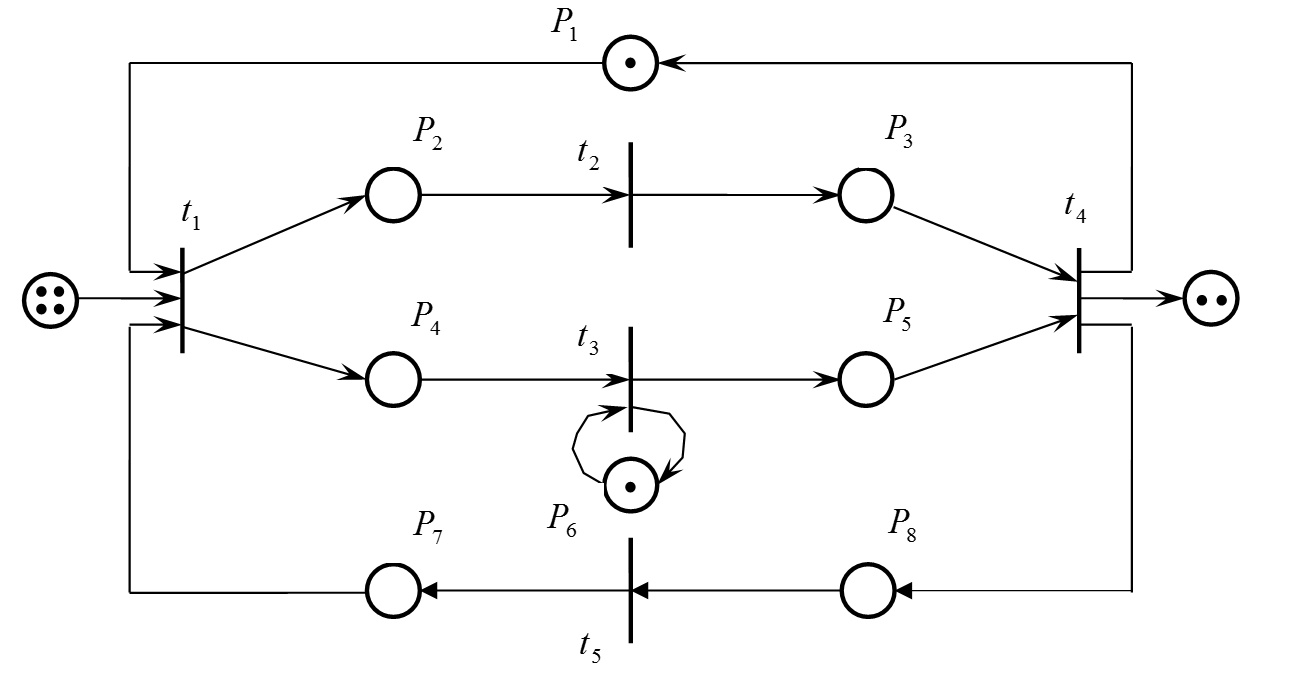
\includegraphics[width=0.7\textwidth]{petri-net}}
	\caption{Пример сети петри.}
	\label{img:petri-net}
\end{figure}

Сетью Петри принято называть тройку $<G, m_0, \rho>$  , где  $G\equiv<P, T, I, O>$ "--- граф сети Петри, $P$   "--- конечное множество позиций (или мест) сети, $T$ "--- конечное множество переходов сети, $P \cap T = \varnothing$. $I, O:T\rightarrow P^{()}$  "--- функции, задающие комплекты входных и, соответственно, выходных позиций переходов сети (здесь $P^{()}$  "--- множество всевозможных конечных комплектов элементов мно-жества $P$ ). $M \cong P^{()}$ "--- множество всевозможных состояний сети (маркировок).  $m_0 \in M$ "--- начальная маркировка сети, задающая начальное состояние сети, $\rho:T\rightarrow C$ "--- функция раскраски, возможно частичная, где $C$  "--- множество красок.

Сеть называется ограниченной, если $ (\forall p \in P) (\exists k \in \textit{nat}) (\forall m \in \mu_0) (m(p) \leq k)$, то есть множество достижимых в сети маркировок конечно.

Ограниченная сеть Петри $S$ на множестве позиций $P$, $|P|\in \mathbb{N}_0$, может быть представлена следуюзим образом~\cite{falkTheory}:\\ 
$ S \subseteq P^{()} \times (P^{()} \times P^{()}) $.

Неограниченная сеть Петри $S$ на  $P$, $|P|\in \mathbb{N}_0$:	$ S \subseteq P^{()} \times 2^{P^{()} \times P^{()}} $.

Для любой сети Петри $S\equiv < m_0, T >,\;  m_0 \in P^{()}$ называется начальной разметкой сети, а направленное квазиотношение $T$ -- множество переходов сети.

Сети Петри рассматриваются с точностью до изоморфизма: две сети $S'\equiv<{m'}_0, T'>$ на $P'$ и $S''\equiv<{m''}_0, T''>$ на $P''$ изоморфны ($ S' \sim S'' $), если существует взаимооднозначное соответствие $ \varepsilon:P'\leftrightarrow P'' $, такое, что $ \varepsilon(T') = T'' $. Графическое представление сетей Петри хорошо известно и не нуждается в уточнении.

Бинарное отношение $\mathrm{T}(T)$ изменения разметок на множестве $P^{()}$ разметок сети Петри $S\equiv < m_0, T >$:
\begin{center}
	$\mathrm{T}(T)\cong\{<p',p''-p_1+p_2>|<p_1,p_2> \in T \wedge p_1\leq p''\}.$
\end{center}

История поведения стандартной ограниченной сети Петри $S\equiv < m_0, T >$: кортеж $<m_0,m_1,...,m_k>$, 
такой, что $(\forall i \in 1..k)(<m_{i-1}, m_i> \in \mathrm{T}(T))$.

Множество всех возможных историй поведения сети Петри $S$ обозначим $\mu(S)$.

Две сети Петри $S_1$ и $S_2$ эквивалентны, если $\mu(S_1) \sim \mu(S_2)$ (т.е. существует взаимно-однозначное соответствие $\varepsilon:P'\leftrightarrow P''$, такое, что $\varepsilon(\mu(S')) = \mu(S'')$).


В качестве графического средства сети Петри могут использоваться для наглядного представления моделируемой системы. 
Вводимое в этих сетях понятие фишек позволяет моделировать динамику функционирования систем и параллельные процессы. 
В качестве математического средства аналитическое представление сети Петри позволяет составлять уравнения состояния, алгебраические уравнения и другие математические соотношения, описывающие динамику систем~\cite{radioElect}.

\section{Сети Петри со строгой дисциплиной изменения разметок}
Бинарное отношение $\bar{\mathrm{T}}(T)$ строгого изменения разметок на множестве $P^{()}$ 
разметок сети в сети Петри $S\equiv < m_0, T >$~\cite{falkTheory}:
\begin{equation}
\begin{multlined}
\bar{\mathrm{T}}(T)\cong\{<p',p''-p_1+p_2>|<p_1,p_2> \in T \wedge p_1\leq p'' \wedge\\
\wedge (\exists<{p'}_1, {p''}_2> \in T)(p_1 < {p'}_1 \wedge {p'}_1 \leq p'') \}.
\end{multlined}
\end{equation}

История поведения ограниченной сети Петри $S\equiv < m_0, T >$ со строгим изменением разметок: кортеж  $<m_0, m_1, ..., m_k>$, 
такой, что\\ $(\forall i \in 1..k)(<m_{i-1}, m_i> \in \bar{\mathrm{T}}(T))$.

Пусть задана стандартная ограниченная сеть Петри $S\equiv < m_0, T >$. Пополним множество $P$ ее позиций множеством $P_G$ новых элементов,
взаимно-однозначно соответствующих переходам из $G$: $P'\cong P\cup P_G$,\\ 
$P_G\cong \{p_t|(t\in T)\wedge (p_t \notin P)\}$. Искомую ограниченную сеть Петри со строгой дисциплиной изменения разметок 
обозначим $S'\equiv  < {m'}_0, T >$:\\
${m'}_0\cong m_0 +\displaystyle\sum_{p_t\in P_G}c_{p_t}$,
$T'\cong\{\alpha'+c_{p_{<\alpha', \alpha''>}}, \alpha'' +c_{<p_{\alpha', \alpha''>}}|<\alpha', \alpha''> \in T\} $.
Доказательство эквивалентности сетей $S$ и $S'$ очевидно.
\section{Динамические вычислительные сети}
% Для отображения символа в большом варианте использовать \displaystyle
Пусть 
$ D = \displaystyle\bigcup_{\theta\in\Theta} D_\theta $  - многосортный \textit{универсум данных},  
где $\Theta$ - конечное множество \textit{сортов} данных, 
$D_\theta$ - подмножество \textit{данных} сорта $\theta\in\Theta$.\\
Будем считать, что одним из таких сортов данных является сорт \textit{nat}, такой, что $D_{\textit{nat}} \cong \mathbb{N}_0$.
Функциональным базисом будем называть конечное множество  $ B $   всюду определенных вычислимых~\cite{falkTheory} функций вида:\\
$ \beta: \displaystyle\bigtimes_{i'\in 1..m'}D_{\theta'_{i'}} \rightarrow \displaystyle\bigtimes_{i''\in 1..m''}D_{\theta''_{i''}} $, $ m', m'' \in \mathbb{N}_0 $  , 
где  $ <m', m''> $   называется арностью функции $ \beta $  , а  $ <\nu', \nu''> $ -- ее типом, где $ \nu'\in \Theta^{<m'>}, \nu''\in \Theta^{m''} $
.

\textit{ Динамической вычислительной сетью} (\textbf{ДВС}) в функциональном базисе $B$ 
назовем пару $<\bar{\Sigma}, \dot{S}>$, где $\overline{\Sigma}$ 
- конечное множество классов сетей ДВС, $\dot{S}$ - аксиома ДВС.

Каждый класс $\Sigma$ характеризуется: 
уникальным именем  $\dot{\Sigma}$, 
типом функции 
$< |\bar{\theta}'(\dot{\Sigma})|, |\bar{\theta}''(\dot{\Sigma})|>$
,  и конечным упорядоченным множеством $S^*(\dot{\Sigma})$
\textit{образов сетей} этого класса.
Тип или арность может указываться,
при необходимости, в виде правого верхнего индекса.

Все образцы сетей из $S^*(\dot{\Sigma})$ имеют тот же тип, а, следовательно,
и арность, что и сам класс $\Sigma$.
Тип или арность образца сети   $S\in\bar{S}(\dot{\Sigma})$ ,
при необходимости, также может указываться в виде его правого верхнего индекса.

Образец сети  $S\in{S^*(\dot{\Sigma})}$   в общем случае имеет вид:
\begin{center}
	$S\cong<P, \delta, I, O, T_T, T_H, \nu', \nu'', I_T, O_T, \sigma, \rho, \varphi_T, \lambda_I, \lambda_O, \mu_0> $,где
\end{center}
\begin{itemize}
	\item $P$ 
	"--- конечное множество элементов\footnote{Используемый здесь термин «элемент сети» является, во многом, аналогом терминов «позиция» или «место» в теории сетей Петри и «точка сети» в теории направленных отношений.}
	образца сети,
	
	\item $\delta:P \rightarrow \Theta$  "--- задает сорта элементов образца сети,
	\item  $I, O \in P^{<>}$ "--- кортежи входных и выходных элементов образца сети, \mbox{$<\delta(I), \delta(O)>$}  "---  тип, а $<|I|, |O|>$   "--- арность образца сети,
	
	\item $T_T$ 
	"--- конечное множество терминальных переходов,
	
	\item $T_H$ 
	"--- конечное множество нетерминальных переходов,
	$T_T \cap T_H = \varnothing$  , $T\cong  T_T \cup T_H$ , $T \cap P = \varnothing$ ,
	
	\item	для всех $ t \in T$  : $I_T(t) \in P^{<\nu'(t)>}$ ,
	$ O_T(t) \in P^{\nu''(t)} $  ;\\
	$<\nu'(t), \nu''(t)>$   "--- \textit{арность перехода}  $ t \in T $   ( $ \nu', \nu'':T\rightarrow\mathbb{N}_0 $ ),\\
	$ <\delta(I_T(t)), \delta(O_T(t))> $  "--- \textit{тип перехода} $t$  , 
	
	\item $ \sigma:T_H \rightarrow \{ \dot{\Sigma}\;| \;\Sigma \in \bar{\Sigma} \} $ (сопоставляет имена классов сетей-объектов нетерминальным переходам),
	
	\item $ \rho:T_H \rightarrow \mathbb{Q}_0 $ (задает \textit{временные сдвиги} для нетерминальных переходов),
	
	\item $ \omega:T_H \rightarrow P $(задает \textit{управляющие входы} нетерминальных переходов), для всех  $ t \in T_H $  $ \delta(\omega(t)) = \textit{nat} $   ;
	
	\item $ \varphi_T:T_T \rightarrow B $ – \textit{семантика} терминальных переходов, причем для всех  $ t \in T_T $    тип  $\varphi_T(t)$    равен  $ <\delta(I_T(t)), \delta(O_T(t))> $  ,
	
	\item $ \lambda_I:\{ <t, i'>|\; t\in T_T \wedge i' \in 1..\nu'(t) \} \rightarrow \mathbb{Q}_0 $ и
	
	\item $ \lambda_O:\{ <t, i''>|\; t\in T_T \wedge i'' \in 1..\nu''(t) \} \rightarrow \mathbb{Q}_0 $ задают «задержки» входных и выходных связей терминальных переходов с элементами образца сети,
	
	\item $ \mu_0 \in M_S $ , 
	где $ M_S \cong \{ \mu\;| \; (\forall p \in P)(\mu(p) \in (D_{\delta(p)} \times \mathbb{Q}_0)^{()} \} $.
	Компонент $ \mu_0 $    является, в определенном смысле, аналогом понятия маркировки сетей Петри,
	в связи с чем множество  $ M_S $   будем тоже называть \textit{множеством возможных маркировок} сети,
	а $\mu_0$   – ее \textit{начальной маркировкой}.
	Не ограничивая общности, далее будем считать, что для любой маркировки  $\mu\in M_S$
	все комплекты  $\mu(p)$  (для всех $p \in P$ ) представлены кортежами вида 
	$ < <d_1, \tau_1>, ..., <d_{|\mu(p)|}, \tau_{|\mu(p)|} > $  , 
	построенными из элементов соответствующего комплекта так, 
	что компоненты кортежей упорядочены по неубыванию вторых компонентов пар 
	(т.е. $ (\forall i\in 1..|\mu|-1) (\tau_i \leq \tau_{i+1}) $~). 
\end{itemize}

\newtheorem{com}{Замечание}
\begin{com}\label{izomorph}
	Заметим, что образцы сетей рассматриваются с точностью до $(P, T_T, T_H)$-изоморфизма.
\end{com}

\textit{ Аксиома} или, по-иному, инициальное состояние $\dot{S}$ ДВС (корень дерева состояний) -- один из образцов некоторого класса $\Sigma \in \bar{\Sigma}$.


\section{Процессы реального времени}
Абстрактный процесс в системе определяется как последовательность $ \langle P_0, P_1, ...\rangle $   состояний системы, а процесс реального времени – как последовательность упорядоченных пар $ \langle P_i, t_i \rangle, i\in N_0 $\footnote{$ \mathbb{N}_0 \cong \{0, 1, 2, \dots\}$}, представленных состояниями системы и временами переходов системы в эти состояния, причем времена в последовательности строго упорядочены по возрастанию. 
Далее мы будем рассматривать только процессы реального времени. 
В общем случае для недетерминированных систем процессы представлены конечными или бесконечными путями из корня дерева процессов.
Корень дерева процессов представляет собой пару $ \langle P(t_0), 0 \rangle $ , где $ P_0 $  – начальное состояние всех заданных этим деревом процессов в момент времени  $ t_0 = 0 $. 

\subsection{Шкала времени} \label{sec:time}
В понятии процесса используется понятие времени, как абстрактного, представленного номерами в образующей процесс последовательности, так и реального, представленного элементами числовой шкалы времени, которая представлена линейно упорядоченным множеством моментов времени и, желательно: 
\begin{itemize}
	\item включает минимальное и максимальное значения, 
	\item имеет разрешимые предикаты сравнения ($ <, \leq, =, \geq, > $),
	\item является плотной, в которой для любых различных моментов времени $ t^{'} $  и $ t^{''} $  , таких, что $ t^{'}<t^{''} $ , существует момент времени $ t $ , такой, что  $ t^{'}<t $  и $ t<t^{''} $ .
\end{itemize}

Не ограничивая общности, будем в качестве удовлетворяющей этим требованиям шкалы времени рассматривать множество $ \breve{\mathbb{Q}} = \mathbb{Q} \cup \{\omega\} $, где $ \mathbb{Q}=\mathbb{Q}_+\cup \{0\} $, $ \mathbb{Q}_+ $~- множество положительных рациональных чисел, $ 0 $ - минимальное значение:$ (\forall t \in \mathbb{Q}_+) (0<t) $ , $ \omega $ - несобственное значение, время, неограниченно отдаленное в будущем: $ (\forall t \in \mathbb{Q}) (t<\omega) $. 
Сохраняя основные свойства арифметических операций, доопределим естественным образом для элементов множества $ \breve{\mathbb{Q}} $ указанные отношения $ <, \leq, =, \geq, > $ и арифметические операции сложения, вычитания, умножения и деления, за исключением некоторых случаев: $ \omega/\omega $ , $ 0/0 $ , $ 0*\omega $  и вычитания из меньшего значения большего. 
Заметим, что положительные рациональные числа представляются упорядоченными парами положительных натуральных чисел, в общем случае неоднозначно. Каноническое представление предполагает, что эти числа являются взаимно-простыми. Через $ \tau $   будем далее обозначать текущее время в системе, через $ t\in \mathbb{Q} $  --- произвольный момент времени.

\section{Понятие эпизода}
В основе предлагаемых далее определений мы используем понятие эпизода. 
Эпизоды задаются их типами и двумя моментами времени: начала и завершения (более точно определено ниже). 
Неформально, эпизоды~--- некие сущности (объекты, свойства и т.п.) на интервалах рассматриваемой шкалы времени. 
Интервал~--- упорядоченная пара $ \langle t^{'}, t^{''}\rangle $ моментов времени, такая, что  $ t^{'}<t^{''} $. 
Состояние системы в любой момент времени $ t $ определяется как неупорядоченный набор (комплект, конечное мультимножество) не завершившихся к этому времени эпизодов.

Пусть $ \phi \equiv \langle e, \theta \rangle $~--- эпизод. 
Первый компонент представляет тип эпизода из не более чем счетного множества  $ E $  типов эпизодов в рассматриваемой системе. 
Важную роль в описании частных случаев определения процессов в системах играет структуризация множества типов эпизодов. 
Разбиение типа на два компонента практически не ограничивает общности: $ E \equiv E_B \times E_D $. 
Первый компонент типа определяет возможные события в системе, приводящие к изменению ее состояния, а второй~--- наполняет их конкретным содержанием. 
Для всех  $ \langle e_B, e_D \rangle \in E $  полагаем, что $ e_B $~--- структурный атрибут эпизода, $ e_D $~--- его информационный атрибут. 
Практически полезной является и дальнейшая детализация структурного атрибута: полагаем, что $ e_B \equiv \langle e_B^{'}, e_B^{''} \rangle $ , где $ e_B^{'} $~--- один из группирующих эпизоды контейнеров, к которому <<относится>> (или, иначе говоря, в котором <<находится>> эпизод), а $ e_B^{''} $~--- сорт (или тег) эпизода, уточняющий средства оперирования с информационными атрибутами (аналог понятия типа или класса информационных объектов в языках программирования). 
В частном случае, сорт эпизода может однозначно определяться его контейнером. 
В свою очередь, сорт эпизода определяет множество возможных значений его информационного атрибута. 
Предполагается, что множество значений информационного атрибута любого сорта содержит неопределенное значение  $ \perp $.

Второй компонент эпизода $ \theta \equiv \langle t^{'} t^{''} \rangle \in \mathbb{Q} \times \breve{\mathbb{Q}} $, $ t^{'}<t^{''} $ задает временные характеристики конкретного эпизода: $ t^{'}\in \mathbb{Q} $  определяет начало эпизода на шкале времени; $ t^{''}\in \breve{\mathbb{Q}} $ , если эпизод завершен ($ \tau \geq t^{''} $), то это --- конец эпизода, иначе эпизод полагается незавершенным, и $ \delta \cong t^{''}-t^{'} > 0 $ понимается как предельно возможная длительность незавершенного эпизода (если $ t^{''}=\omega $ , то возможная длительность эпизода сверху не ограничена). 

\section{Состояние вычислительной системы}

Пусть $ D = \bigcup_{\theta \in \Theta} D_\theta $ - многосортный универсум данных, где $ \Theta $ - конечное множество сортов данных, $ D_\theta $ - подмножество данных сорты $ \theta \in \Theta $.

\textit{Структура вычислительной сети} $ S = \langle C, I \rangle $ представляет собой пару множеств. 

Первое из них, $ C $ --- множество контейнеров эпизодов. 
Контейнер $ c \in C $ определяется множеством сортов эпизодов, допустимых для помещения в контейнер.

Второе множество, $ I $ - интерфейс системы. 
Интерфейс состоит из элементов интерфейса и определяет возможные изменения в системе. 
Элемент $ i  = \langle \beta, R \rangle $ представляет собой пару из функции функционального базиса $ \beta \in B $ (определим его далее) и множества требований к атрибутам эпизодов, необходимых для срабатывания элемента интерфейса.
Для всех $ \langle r_B, r_T \rangle \in R $ полагаем, что $ r_B $ - требование к структурному атрибуту эпизода (к контейнеру и (или) сорту), а $ r_T \in \mathbb{Q}_+ $ - требуемое минимальное время жизни эпизода по отношению к текущему моменту времени $ \tau $.

\textit{Состоянием вычислительной сети} в момент времени $ t \in \mathbb{Q} $ называется $ P_t = \langle E_t, S_t \rangle $, где
\begin{itemize}
	\item $ E_t $ --- множество незавершенных эпизодов в момент времени $ t $;
	\item $ S_t $ --- структура вычислительной системы в момент времени $ t $.
\end{itemize}


\section{Интерфейс системы}
Согласно нашему первоначальному замыслу, основные объекты в определении понятия системы~--- состояние системы, интерфейс, элемент интерфейса – должны были быть определены как неупорядоченные наборы, соответственно, незавершенных эпизодов, элементов интерфейса и требований к структурным атрибутам эпизодов, необходимых для срабатывания элементов интерфейса, составляющих события в системе, приводящие к изменению ее состояния. 
Однако, вследствие этого появляется значительная неопределенность в поведении системы, выражающаяся в чрезмерном разрастании дерева процессов. Для предотвращения этого мы отказались от концепции неупорядоченности, что позволило ввести в описание систем разного рода приоритеты, устраняющие во многом недетерминированность поведения систем. 
Фактически, неоднозначность появляется только вследствие маловероятного случайного совпадения времени готовности к срабатывания структурно не связанных элементов интерфейса и по причине сознательного отказа от учета информационных атрибутов эпизодов в формировании событий в системе, оставив только их влияние на результат~--- возможные изменения состояния системы.

В дальнейшем будем различать два варианта систем: с последовательным и параллельным интерфейсом.

В общем случае интерфейс рассматривается как упорядоченное множество элементов интерфейса, причём требование упорядоченности используется, во-первых, для приоритетного применения элементов интерфейса для систем с последовательным интерфейсом, во-вторых, для приоритетного распределения эпизодов состояния системы при одновременном срабатывании комплекта элементов интерфейса для систем с параллельным интерфейсом.

\subsubsection{Дисциплины выбора эпизодов}
Каждый отдельный элемент интерфейса определяет кортеж требований к элементам соответствующего ему набора эпизодов, а именно, к их контейнерам и (или) сортам, а также к временам их появления (к началам эпизодов) по отношению к минимально возможному моменту предполагаемого их совместного срабатывания – в виде так называемой <<выдержки>> эпизодов с областью значений $ \mathbb{Q}_+ $ . 
Если из эпизодов текущего состояния системы можно сформировать соответствующий элементу интерфейса кортеж эпизодов, то будем говорить, что элемент интерфейса готов к срабатыванию в рассматриваемый момент времени. 
Ограничить разнообразие удовлетворяющих этим требованиям комплектов эпизодов можно дополнительно заданием для конкретного элемента интерфейса одной из дисциплин выбора эпизодов из текущего состояния системы: 
\begin{itemize}
	\item \textit{FIFO} (First In First Out) --- предпочтение отдается <<старым>> эпизодам (с более ранним началом);
	\item \textit{LIFO} (Last In First Out) --- предпочтение отдается <<молодым>> эпизодам (с более поздним началом);
	\item \textit{FEFO} (First End First Out) --- предпочтение отдаётся эпизодам с более ранним временем окончания.
\end{itemize} 

\subsection{Задание интерфейса}

В простейшем случае элементы действующего в текущий момент времени интерфейса могут быть заданы путем их непосредственного перечисления, разумеется, если их конечное число.
В более общем случае, который в этой работе не рассматривается, интерфейс задается в форме некоторой схемы – выражений формального языка, содержащих, возможно, свободные вхождения переменных с известными областями значений, причем возможными значениями этих выражений являются отдельные элементы интерфейса, а само множество значений является рекурсивно-перечислимым (и, в общем случае, может быть бесконечным). 

\subsection{Последовательные и параллельные интерфейсы}

Для систем с последовательным интерфейсом отдельные его элементы анализируются на возможность срабатывания в порядке их перечисления, вплоть до первого готового к срабатыванию в ближайший момент времени по отношению к времени предыдущего события. 
Очевидно, что \textit{в один и тот же момент времени может произойти последовательное срабатывание нескольких элементов интерфейса} в порядке их перечисления.

Для систем с параллельным интерфейсом отдельные элементы интерфейса определяют только возможность событий в системе. 
В системе выделяются готовые к одновременному срабатыванию в некоторый момент времени подкомплекты эпизодов текущего состояния системы при условии ненаступления до этого других событий. 
Поэтому переход к новому состоянию системы, как и для систем с последовательным интерфейсом, может стать реальным только для возможных событий с минимальным ожидаемым временем. 
Если это время окажется больше максимально возможного времени окончания хотя бы одного из выбранных эпизодов, то для определения готовности всё следует повторить для состояния, в котором удалены такие эпизоды. 
Если требуемых комплектов эпизодов нет, то процесс завершается; в противном случае рассматривается готовность к одновременному срабатыванию всевозможных комплектов указанных комплектов эпизодов для отдельных элементов параллельного интерфейса. 
Хотя при этом рассматривается возможность выделения в состоянии системы комплектов эпизодов на основе <<смешивания>> упорядоченных по времени выдержки подкортежей требований к различным значениям структурных атрибутов эпизодов, необходимых для срабатывания элементов интерфейса, однако, сам выбор конкретных эпизодов и сама возможность такого выбора с полученным на первом этапе минимально возможным временем срабатывания могут оказаться иными даже при условии сохранения дисциплины выбора, индивидуально заданной для каждого элемента интерфейса. 
Полагаем, что фактически смогут реализоваться только \textbf{максимальные} из этих готовых к совместному срабатыванию комплектов элементов интерфейса. 
Реализуемый таким образом \textit{принцип максимально возможного параллелизма} в поведении системы позволяет исключить из рассмотрения события с одним и тем же временем. 
Если таких максимальных суммарных комплектов более одного, то поведение системы становится недетерминированным, и, как было сказано ранее, оно формализуется в виде дерева процессов: происходит его ветвление, вершина текущего состояния системы будет иметь несколько потомков, по одному для каждого указанного выше случая. 
Каждый из вариантов определяет и свой результат соответствующего события, т.е. изменения состояния системы и действующего интерфейса.

\section{События}
Изменение состояний системы в автоматной модели определяется как ее текущим состоянием, так и действующим интерфейсом, который устанавливает взаимосвязь эпизодов и, в общем случае, сам тоже может изменяться при переходах системы к новым состояниям. В каждый момент времени действующий интерфейс определяет для текущего состояния системы возможность событий, в результате которых могут измениться и состояние системы, и действующий интерфейс. 
Событие~--- переход системы в новое состояние, который характеризуется моментом времени этого перехода и определяется временем ближайшего предшествующего события, текущим состоянием системы и действующим интерфейсом эпизодов. 
Первопричинами основных событий являются: 
\begin{enumerate}[label=\arabic*)]
	\item появление в состоянии системы наборов (комплектов) эпизодов, необходимые требования к которым и определяет действующий интерфейс;
	\item в динамических системах~--- подключение к системе определенным образом модифицированных копий подсистем. 
\end{enumerate}
Изменение состояния системы возможно также в связи с достижением максимально возможного времени окончания некоторого эпизода, в этом случае такой эпизод исключается из состояния системы и не может влиять на последующие события. 
Информационный атрибут такого завершенного эпизода полагается равным $ \perp $. 

\section{Результат события}
Перейдем к краткому рассмотрению результата события – к изменениям состояния системы.

Пусть процесс не обрывается и $ t_{i+1} $  – время очередного события. 
Во-первых, из состояния $ P_i $ уже исключены эпизоды, время максимально возможного окончания которых меньше $ t_{i+1} $. 
Участвующие в событии эпизоды также исключаются из состояния системы. 
Каждый из участвовавших в событии элемент интерфейса порождает, с учетом его кратности вхождения в реализованный в событии комплект элементов интерфейса, комплект новых эпизодов, добавляемых к текущему состоянию системы (после указанных выше удалений эпизодов). 
Для каждого нового эпизода задаются полностью (и контейнеры, и сорта) структурные атрибуты, <<задержка>> (число из $ \mathbb{Q} $ ), результат сложения которого с  $ t_{i+1} $  дает начало этого эпизода, и еще одно число из $ \breve{\mathbb{Q}} $ . 
Если оно равно нулю, то длительность нового эпизода не ограничена сверху (параметр <<конец эпизода>> получает значение $ \omega $ ), в противном случае он задает положительную длительность эпизода, а значение параметра <<конец эпизода>> получается сложением длительности с началом эпизода. 
Все это, в сочетании с требованием задания положительных значений для выдержек, гарантирует отсутствие готовности к срабатыванию в момент времени $ t_{i+1} $ новых, появившихся в результате рассматриваемого события, эпизодов в состоянии системы. 

\subsection{Функциональный базис системы}
В общем случае все характеристики новых эпизодов определяются как значения заданных для каждого элемента интерфейса функций из функционального базиса системы, согласованных по сортам аргументов с сортами входных эпизодов элемента интерфейса. 
Значениями аргументов этих функций выступают значения информационных атрибутов выделенных в состоянии системы $ P_i $ участвующих в событии эпизодов для рассматриваемого элемента интерфейса. 
Именно с целью установления соответствия аргументов и их значений перечисление требований к эпизодам уже в элементе интерфейса осуществляется в некотором порядке, т.е. в форме кортежа. 

В частном случае, структурные атрибуты (контейнеры, сорта) и максимально возможные времена окончаний новых эпизодов задаются непосредственно в элементе интерфейса, если всем сортам эпизодов сопоставлены одноэлементные множества возможных значений информационных атрибутов. 

Существует несколько альтернатив определения функции в функциональном базисе, которые зависят от параметров системы.
\begin{itemize}
	\item Функции вида $ \beta : \bigtimes_{i \in 1..n} D_{\theta_i} \rightarrow \bigtimes_{i \in 1..m} D_{\theta_i}$, где $ \langle
	n,m \rangle $ - арность функции, а $ \langle \nu, \mu \rangle $ - тип функции, где $ \nu \in \Theta^{<n>}, \mu \in \Theta^{<m>} $. 
	Такие функции лишь выполняют вычисления с использованием информационных атрибутов. 
	Результат функции --- кортеж новых информационных атрибутов фиксированной длины. 
	Для создания новых эпизодов элемент интерфейса должен также содержать кортеж связей элемента с контейнерами результатов $ <c, t_l, t_d >, c \in C, t_l \in \mathbb{\mathbb{Q}}_+, t_d \in \mathbb{\mathbb{Q}} $, где $ c $ - контейнер результата, $ t_l $ - время задержки эпизода, $ t_d $ - длительность эпизода.
	\item Функции вида $ \beta : \bigtimes_{i \in 1..n} D_{\theta_i} \rightarrow \bigtimes_{i \in 1..m} (D_{\theta_i} \times \mathbb{Q}_+ \times \mathbb{Q})$. 
	В отличае от предыдущего вида, время задержки эпизода и длительность эпизода здесь определяется функцией.
	Элемент интерфейса же содержит исключительно информацию о целевых контейнерах для результатов функции.
	\item Функции вида $ \beta : (\bigtimes_{i \in 1..n} D_{\theta_i}) \times \mathbb{Q}_+ \rightarrow \bigtimes_{i \in 1..m} \Phi_{\theta_i}$, где $ \Phi $ - множество возможных эпизодов.
	В качестве последнего входного параметра используется $ \tau $ - текущее время в система.
	Заранее неизвестно, в какой контейнер попадёт новый эпизод, однако сохраняются арность и тип функции.
	\item Функции вида $ \beta : (\bigtimes_{i \in 1..n} D_{\theta_i}) \times \mathbb{Q}_+ \rightarrow \Phi^{\langle\rangle}$.
	Для таких функций возможно не только определять значение структурного атрибута результатов, но и управлять своей арностью.
\end{itemize}

\subsection{Изменение структуры}
Описанные события не приводят к изменению структуры системы, множество используемых контейнеров ограничено множеством контейнеров, фигурирующих в начальном состоянии системы и ее интерфейсе. 
Такие системы будем называть статическими. 
Для описания поведения динамических систем, интерфейс которых может изменяться во времени, а множества используемых контейнеров неограниченно расширяться, нужны совсем иные пути формализации для реализации этих возможностей. 
Не претендуя на общность, мы предлагаем дополнительно ввести в качестве элементов интерфейсов динамических систем так называемые нетерминальные элементы, в то время как рассмотренные ранее будем называть терминальными элементами интерфейсов. 

Если для терминальных элементов интерфейса эффект выражается в создании новых эпизодов и сохранении действующего интерфейса, то в результате срабатывания нетерминального элемента интерфейса происходят структурные изменения: могут появиться новые элементы интерфейса, могут появиться не только новые эпизоды в состоянии системы, но и новые контейнеры. 
Вопрос же об удалении из рассмотрения некоторых контейнеров и элементов интерфейса должен решаться подобно тому, как решается проблема <<сборки мусора>> для памяти типа <<куча>>.

Динамическая система представлена в виде конечного множества именованных подсистем, каждая из которых задана тройкой~--- начальным состоянием, начальным интерфейсом и упорядоченным конечным подмножеством контейнеров подсистемы, элементы которого будем называть контактами подсистемы. 
Контейнеры подсистемы, не вошедшие в число контактов, при срабатывании нетерминального элемента интерфейса и подключении к системе этой подсистемы будут представлять новые контейнеры, отличные от всех ранее используемых в системе. 
Механизм порождения новых контейнеров аналогичен процессу выделения новых ячеек в памяти типа <<куча>> и, в какой-то мере, операции замены связанной переменной в формальных системах с операторами, связывающих вхождения операторной переменной в терм, к которому применяется оператор (например в $ \lambda $-исчислении). 
Вершина дерева процессов (начальное состояние системы) представлена начальным состоянием выделенной базовой подсистемы (аксиомы). 
Предполагается возможность в дальнейшем подключений к системе любых подсистем, в том числе и подсистемы-аксиомы. 
Множество имен всех подсистем образуют особый сорт $ \Delta $ значений информационных атрибутов эпизодов.

В текущем интерфейсе всякий нетерминальный элемент представлен следующей информацией: 
\begin{enumerate}[label=\arabic*)]
	\item контейнером, наличие в котором эпизода сорта $ \Delta $   может привести к срабатыванию этого нетерминального элемента, 
	\item  выдержкой, играющей ту же роль, что и выдержки эпизодов в терминальных элементах интерфейса, 
	\item  кортежем контейнеров текущего состояния системы, элементы которого будем называть контактами рассматриваемого нетерминального элемента текущего интерфейса (заметим, что один и тот же контейнер может входить неоднократно в указанный кортеж), 
	\item  функцией, аргументом которой является имя подсистемы, а значением – задержка подключения соответствующей подсистемы из множества $ \mathbb{Q} $ .
\end{enumerate}  

Условием возможного срабатывания нетерминального элемента интерфейса в момент времени $ t_{i+1} = t_i + \delta $, где $ \delta $~--- указанная для этого элемента <<выдержка>>, является просто наличие в состоянии системы соответствующего эпизода сорта $ \Delta $ в указанном контейнере. 
В результате срабатывания нетерминального элемента интерфейса происходит подключение к системе некоторой подсистемы, имя которой определяется информационным атрибутом эпизодов, что приводит к изменениям основных компонентов состояния системы, помимо тех, которые вносятся в результате возможного одновременного срабатывания терминальных элементов интерфейса. 
Одна из основных проблем определения процедуры подключения подсистемы состоит в том, чтобы она исключала возможность в момент времени подключения срабатывания новых элементов обновленного интерфейса. 
Кроме того, при одновременном срабатывании нескольких нетерминальных элементов результат подключения нескольких подсистем не должен зависеть от порядка их реализации.

\subsection{Подключение подсистемы}
Опишем вначале способ подключения к системе некоторой одной подсистемы.

Как было сказано ранее, для выполнения подключений каждая подсистема, помимо ее начального состояния и начального интерфейса, содержит контактную информацию для ее подключений, и, в свою очередь, всякий нетерминальный элемент действующего интерфейса системы также содержит свою контактную информацию. 
Контактная информация позволяет установить связь между контейнерами основной системы и контейнерами подключаемой подсистемы путем замены контейнеров в подключаемой системе на соответствующие (согласно порядкам перечисления контактов) контейнеры основной системы; 
именно для того, чтобы при подключении не возникла возможность <<ложных>>, не реализованных к моменту подключения срабатываний элементов действующего интерфейса системы, соответствующая контактная информация в основной системе задается в форме кортежа используемых в ней контейнеров, а в подключаемой подсистеме --- в форме упорядоченного подмножества используемых в ней контейнеров, причем для остальных контейнеров подключаемой подсистемы производится их замена на новые контейнеры, не используемые ранее в основной системе. 
При подключении подсистемы начала всех эпизодов во всех ее контейнерах формируются путем сложений их начал и, соответственно, концов, заданных в начальном состоянии подключаемой подсистемы, времени события, включающего срабатывание рассматриваемого нетерминального элемента основной системы, и задержки подключения соответствующей подсистемы при срабатывании конкретного нетерминального элемента интерфейса системы. 
Так как новый интерфейс системы в результате срабатывания нетерминального элемента пополняется элементами интерфейса подключаемой подсистемы, то указанное изменение временных параметров подключаемых к состоянию системы эпизодов подсистемы не может привести к готовности в тот же момент времени к срабатыванию как <<старых>>, так и <<новых>> элементов интерфейса. 
Очевидно, что, так как интерфейс подключаемых подсистем может тоже содержать нетерминальные элементы, то в системе может неограниченно увеличиваться количество используемых контейнеров и элементов интерфейса, а описанная далее <<сборка мусора>> в системе может приводить к удалению <<лишних>> эпизодов, контейнеров и элементов интерфейса.

В общем случае, событие, приводящее к изменению состояния системы в момент времени $ t_{i+1} $ , может включать одновременное срабатывание не только нескольких терминальных элементов интерфейса, но и нескольких его нетерминальных элементов. 
Подключение одной подсистемы предполагает следующую последовательность шагов:
\begin{itemize}
	\item создание рабочих копий начального состояния и начального интерфейса выбранной для подключения подсистемы (далее под состоянием и интерфейсом подключаемой подсистемы будем понимать эти копии); 
	изменение в состоянии и интерфейсе подключаемой подсистемы временных параметров эпизодов так, как было описано выше;
	\item замена различных контейнеров в состоянии и интерфейсе подключаемой подсистемы на различные новые контейнеры, не используемые ни в текущем состоянии и интерфейсе системы, ни в начальном состоянии и интерфейсе подключаемой подсистемы;
	\item замена всех контейнеров в состоянии и интерфейсе подключаемой подсистемы, входящих в число ее контактов, на соответствующие им по порядку контейнеры в кортеже контактов рассматриваемого нетерминального элемента интерфейса (если в последнем <<хватает>> контактов);
	\item к состоянию системы присоединяется состояние подключаемой подсистемы (путем сложения представляющих их комплектов), а к интерфейсу систем добавляется интерфейс подключаемой подсистемы (путем конкатенации представляющих их кортежей).
\end{itemize}

\section{Вывод}
Описанная модель является развитием теории Динамических вычислительных сетей, основанной на сетях Петри. 
Однако, в данном формализме предполагается наличие принципиальных отличий даже базовых понятий теории сетей Петри: 
\begin{itemize}
	\item отказ от переходов с пустым комплектом входных позиций: в этом отношении мы обобщаем принцип <<отсутствие необходимых ресурсов (фишек) не может служить основанием каких-либо событий (переходов).>> Это требование, не являясь принципиальным при рассмотрении поведения системы в абстрактном времени, для реального времени является принципиальным;
	\item введение линейных порядков на множествах входных и выходных позиций переходов уже используются во многих обобщениях формализма сетей Петри, и, как следствие, замена понятий <<комплект входных (выходных) позиций перехода>> на понятия <<кортеж входных (выходных) эпизодов для элемента интерфейса>>. В  нашем формализме это необходимо для описания роли информационных атрибутов эпизодов;
	\item срабатывание переходов (элементов интерфейса) управляется не только наличием фишек во входных позициях (контейнерах), а и их окраской (сортами эпизодов);
	\item изменение состояний происходят в реальном, а не в абстрактом (модельном) времени, что позволяет строить более адекватные модели поведения реальных систем;
	\item в нашем подходе всегда реализуется максимально возможный параллелизм срабатывания элементов интерфейса (в базовой модели сетей Петри не допускается одновременное срабатывание нескольких переходов, а моделирование этого делает сеть неоправданно громоздкой). Этот подход позволяет в системе реального времени избавиться от возможности нескольких событий с одинаковым временем;
	\item наконец, главное: сами рассматриваемые нами системы являются динамическими, могут структурно меняться во времени и иметь при функционировании априори не ограниченную сложность.
Изменением терминологии хочется подчеркнуть следующую основную цель публикации: описание проходящих в реальном времени параллельных вычислительных процессов в динамических системах с априори не ограниченной сложностью \cite{Falk}.
\end{itemize}


